\addtocontents{toc}{\vspace{2em}}
\newpage
\section{Maintenance \& Fleet Management}
Maintenance is a key factor in a Public Transport Service company, in particular the aim is to optimize maintenance both for what concern the active maintenance time, but also  for what concerns the reliability of all the rolling stock components.

The traditional KPIs that can generally help to assess the impact of the maintenance in a PTO can be:

\begin{description}
    \item [Unscheduled or scheduled downtime] it helps maintenance managers to analyze how successfully they have implemented maintenance strategies:
        \begin{equation}
            D (\%)= \frac{hour\:of\: unscheduled\:or\:scheduled\:downtime}{total\:time\:period}\cdot 100
        \end{equation}
        And related to that, the downtime affects the cost as:
        \begin{equation}
        D_{cost} (\$/h)= unit\: per\: hour\: \cdot\: profit\: per\: hour
        \end{equation}
    \item [Mean Time Between Failures (MTBF)]
        \begin{equation}
            MTBF = \frac{operating\:time\:hours}{number\:of\:failures}
        \end{equation}
    \item [Mean Time To Repair (MTTR)]
        \begin{equation}
            MTTR = \frac{total\:maintenance\:time}{number\:of\:repairs}
        \end{equation}
    \item [Ratio of Budgeted vs Actual Maintenance Costs] It's possible to categorize the costs into unplanned and planned maintenance, in order to find areas for improvement:
        \begin{equation}
            budgeted\:vs\:actual\:maintenance\:costs = \frac{actual\:maintenance\:cost}{budget}
        \end{equation}    
\end{description}


\subsection{Electric Bus and Infrastructure}
\label{sec:elbusinfra}
Electric buses and generally electric vehicles need their own charging infrastructure depending on their battery’s specification which is highly expensive itself. Building infrastructure for electric buses requires high financing resources and subsidiaries from PTA except if PTO wins a long-term concession. By assuming that PTO undertakes a long-term concession, the most relevant and non-negligible KPIs are gathered.

Here below we mentioned some generic important KPIs, which affect the public, end-users, and PTO commonly, in case of cost, energy, and maintenance related to the bus and its infrastructure including charging in depot and opportunity charging.

\begin{description}
    \item [Total Cost of Infrastructure] which can be divided in the following costs:
        \begin{itemize}
            \item Electric Vehicle + Battery
            \item Opportunity Charging System
            \item Charging point + Charging pole + Installation cost + Smart Charging + ICT Compliance (for charging in depot)
            \item Energy Cost
            \item Electricity Network Losses
            \item Scheduled and unscheduled repair cost of bus, battery, charger and infrastructure
        \end{itemize}
    \item [Energy Consumption] The Energy demand (KWh) can be computed as the the sum of Energy demand for single charging by opportunity charging and the Energy demand for single charging by charging overnight in depot
    
    The Energy consumption of HVAC (KWh) is instead equal to the Energy consumption due to Heating, Ventilation and Air Conditioning system
    \item [Maintenance] The total maintenance time (hours) is equal to the duration of unscheduled and scheduled repair of bus, battery, charger and infrastructure
    
    Total MTBF is the number of failure per operational hours of bus, battery and infrastructure
\end{description}


\subsection{Hydrogen bus and Infrastructure}
As mentioned in \ref{sec:elbusinfra}, it is assumed that PTO wins a long-term concession in which the chance of building the infrastructure gets higher. The most relevant KPIs related to both infrastructure and fuel cell bus were collected.

\begin{figure}[h!]
    \centering
    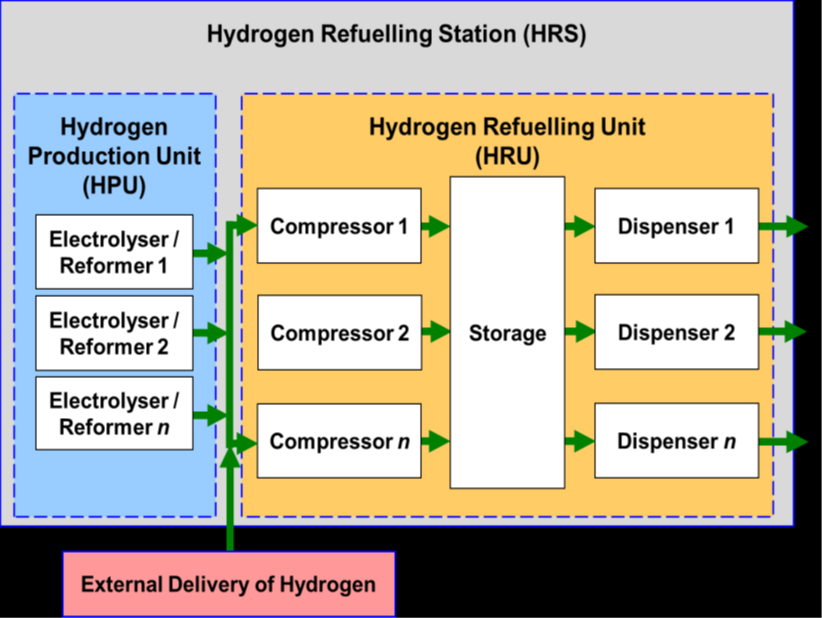
\includegraphics[width=0.6\textwidth]{Images/manteinance/areas_hydrogen.png}
    \caption{Areas covered in hydrogen refueling infrastructure performance assessment }
    \label{fig:areashydrogen}
\end{figure}

In terms of the performance assessment, the hydrogen refueling infrastructure consists of four areas: 

\begin{itemize}
    \item On-site hydrogen production in the HPU (Hydrogen Production Unit)
    \item Hydrogen compression, storage, and dispensing in the HRU (Hydrogen Refueling Unit)
    \item External hydrogen delivery
    \item Aspects related to the operation of the entire HRS (Hydrogen Refueling Station). 
\end{itemize}

The indicators for assessing the performance of the hydrogen refueling infrastructure and its major elements can be found in the following set of tables: 
\begin{itemize}
    \item On-site hydrogen production in the HPU (Table \ref{tab:hpu})
    \item Hydrogen compression, storage, and dispensing in the HRU (Table \ref{tab:hru})
    \item Aspects related to the operation of the entire HRS (Table \ref{tab:hrs})
\end{itemize}

% Please add the following required packages to your document preamble:
% \usepackage{multirow}
% \usepackage{graphicx}
\begin{table}[p]
\centering
\resizebox{\textwidth}{!}{%
\begin{tabular}{|l|l|l|}
\hline
\rowcolor{bluepoli!40}
\multicolumn{1}{|c|}{\textbf{KPI Name}} &
  \multicolumn{1}{c|}{\textbf{period}} &
  \multicolumn{1}{c|}{\textbf{Unit of measure}} \\ \hline
Availability of the HPU &
  \multirow{3}{*}{Monthly, annually and overall} &
  \% \\ \cline{1-1} \cline{3-3} 
\begin{tabular}[c]{@{}l@{}}Amount of hydrogen produced \\ by the HPU and \\ by eachof its electrolysers/reformers\end{tabular}  &  & \%     \\ \cline{1-1} \cline{3-3} 
\begin{tabular}[c]{@{}l@{}}Specific water consumption \\ for hydrogen production\end{tabular} &
   &
  liters/Nm3 or liters/kg \\ \hline
HPU downtime &
  \multirow{2}{*}{Annually and overall} &
  hours \\ \cline{1-1} \cline{3-3} 
\begin{tabular}[c]{@{}l@{}}Specific energy consumption \\ of the HPU and of each \\ of its electrolysers/reformers\end{tabular} &  & kWh/kg \\ \hline
\end{tabular}%
}
\caption{Performance indicators of the HPU}
\label{tab:hpu}
\end{table}
% Please add the following required packages to your document preamble:
% \usepackage{multirow}
% \usepackage{graphicx}
\begin{table}[p]
\centering
\resizebox{\textwidth}{!}{%
\begin{tabular}{|l|c|l|}
\hline
\rowcolor{bluepoli!40}
\multicolumn{1}{|c|}{\textbf{KPI Name}} &
  \textbf{period} &
  \multicolumn{1}{c|}{\textbf{Unit of measure}} \\ \hline
Availabilityof the HRU        & \multirow{2}{*}{Monthly,annually and overall} & \%     \\ \cline{1-1} \cline{3-3} 
HPUdowntime                   &                                               & hours  \\ \hline
Mean timebetween failures     & \multicolumn{1}{l|}{Annuallyand overall}      & hours  \\ \hline
Reliabilityof the HRU         & \multirow{4}{*}{Monthly,annually and overall} & \%     \\ \cline{1-1} \cline{3-3} 
\begin{tabular}[c]{@{}l@{}}Amount ofhydrogen dispensed \\ to the project buses overall and per bus\end{tabular} &
   &
  kg \\ \cline{1-1} \cline{3-3} 
Specificpower consumption HRU &                                               & kWh/kg \\ \cline{1-1} \cline{3-3} 
Speed ofdispensing            &                                               & kg/min \\ \hline
\end{tabular}%
}
\caption{Performance indicators of the HRU}
\label{tab:hru}
\end{table}
% Please add the following required packages to your document preamble:
% \usepackage{multirow}
% \usepackage{graphicx}
\begin{table}
\centering
\resizebox{\textwidth}{!}{%
\begin{tabular}{|l|c|l|}
\hline
\rowcolor{bluepoli!40}
\multicolumn{1}{|c|}{\textbf{KPI Name}} &
  \textbf{period} &
  \multicolumn{1}{c|}{\textbf{Unit of measure}} \\ \hline
\begin{tabular}[c]{@{}l@{}}Specific energy\\  consumption along \\ the on-sitehydrogen supply chain\end{tabular} &
  \multicolumn{1}{l|}{Monthly, annually and overall} &
  kWh/kg \\ \hline
Cost of hydrogen dispensed &
  \multirow{3}{*}{Annually and overall} &
  €/kg hydrogen dispensed \\ \cline{1-1} \cline{3-3} 
\begin{tabular}[c]{@{}l@{}}Number of incidents \\ affecting fuel quality\end{tabular} &
   &
  \# \\ \cline{1-1} \cline{3-3} 
Specific nitrogen consumption &
   &
  kg/tone dispensed \\ \hline
\end{tabular}%
}
\caption{Performance indicators of the HRS}
\label{tab:hrs}
\end{table}
% Please add the following required packages to your document preamble:
% \usepackage{multirow}
% \usepackage{graphicx}
\begin{table}[h!]
\centering
\resizebox{\textwidth}{!}{%
\begin{tabular}{|l|l|l|}
\hline
\rowcolor{bluepoli!40}
\multicolumn{1}{|c|}{\textbf{KPI Name}} & \multicolumn{1}{c|}{\textbf{period}}           & \multicolumn{1}{c|}{\textbf{Unit of measure}} \\ \hline
Scheduled and unscheduled repair cost & Annually and overall & €     \\ \hline
Specific fuel consumption               & \multirow{3}{*}{Monthly, annually and overall} & kg H2/ 100 km                                 \\ \cline{1-1} \cline{3-3} 
Operating hours per fuel cell system  &                      & hours \\ \cline{1-1} \cline{3-3} 
Availability of bus                   &                      & \%    \\ \hline
\end{tabular}%
}
\caption{Performance indicators of FC bus operation and refueling}
\label{tab:fc}
\end{table}

\newpage
\subsection{New Technologies and Fleet Management}
Fleet management KPIs aim at measuring the efficiency of service in many terms. But the most common benchmarks are:
\begin{itemize}
    \item boosting efficiency
    \item enhancing productivity
    \item controlling costs
\end{itemize}

Setting the specific KPIs is one aspect and meeting them is another one. With the exponential growth of technology in this era, applications and software can help to better meet KPIs by collecting real-time data. Here below are listed some fields in which that application can help:

\begin{description}
    \item [Cost Control and Budget Adherence] Because so many costs are associated with fleets, it is difficult to track expenses manually by fleet managers. Fleet managers aim to control expenses and maximize profitability: 
        \begin{itemize}
            \item Real-time cost of ownership tracking and reporting
                \begin{enumerate}
                    \item Create custom reports
                    \item Watching real-time cost per unit of distance information
                    \item Optimize vehicle usage on individual asset trends: by tracking the cost of each vehicle in real-time, you can properly respond to changing market conditions and unpredictable wear and tear.
                    \item Controlling expenses such as fuel, depreciation, fees, maintenance, administrative costs, insurance, etc. 
                \end{enumerate}
        \end{itemize}
    
    Based on the fleet reports it is possible to:
    \begin{itemize}
    \item View operational costs in real-time
        \begin{itemize}
            \item Vehicle operating costs (fuel and service)
             \item Total fleet operating cost by month
             \item Cost per mile (km or hour) trends
        \end{itemize}
    \item Track how your vehicle and equipment are being used
        \begin{itemize}
            \item Average mileage per day (utilization) by vehicle or group
            \item Vehicle assignment history across operators and vehicles
            \item History of status changes (in-shop, out-of-service, etc.)
            \item Audit trail of changes to all asset records (service, parts, issues, etc.)
        \end{itemize}
    \item 	Gain insights into how your assets are being maintained
        \begin{itemize}
            \item Service line items and cost summaries
            \item Scheduled vs. unscheduled maintenance
            \item Downtime reporting
            \item Most common service activities across your fleet
        \end{itemize}
    \item 	fuel consumption trends and efficiency
        \begin{itemize}
            \item Consumption trends by vehicle or group
            \item Fuel-ups by location
        \end{itemize}
    \item Ensure your fleet is safe and compliant
        \begin{itemize}
            \item All inspections completed and by whom
            \item View all reported defects, identify trends 
        \end{itemize}
    \end{itemize}
    \item [Maintenance Management and Downtime Prevention] Prioritizing maintenance productivity reduces downtime and maximizes efficiency. We should track issues by vehicle. Comprehensively tracking vehicle health allows you to spot recurring issues and trends across your vehicles:
    \begin{itemize}
    \item Capture issues as soon as they arise
        \begin{itemize}
            \item Mobile defect reporting
            \item Automated issue reporting
        \end{itemize}
    \item	Take action immediately
        \begin{itemize}
            \item	Coordinate with external shops electronically
            \item	Link vehicle issues to in-house Work Orders
        \end{itemize}
    \item	Collaborate in real-time
        \begin{itemize}
            \item	Mobile notifications
            \item	Interact with team members
        \end{itemize}
    \item	Track resolution and operate smarter
        \begin{itemize}
            \item	Maintain complete audit trail
        \item	Gain insight into your fleet maintenance
        \end{itemize}
    \end{itemize}
    
    To avoid recurring issues, adhering to a preventive maintenance schedule helps identify and repair issues before they compound and cause downtime:
    \begin{itemize}
    \item	Set service schedules and reminders across your fleet
        \begin{itemize}
            \item	Meter and time intervals
            \item Mobile Reminders 
        \end{itemize}
    \item	Save time, increase PM compliance, and reduce breakdowns with Service Programs
        \begin{itemize}
            \item	Keep PM schedules aligned throughout your fleet
            \item	Base Service Programs on OEM guidelines
        \end{itemize}
    \item	Predict when maintenance is due based on usage
    \end{itemize}
    \item [Optimal Vehicle Replacement Targets] Determining the best time to replace a vehicle is complex. Leveraging applications and software to monitor vehicle health and expenses can help identify optimal replacement windows. With these Analysis Tools, fleet managers can take a strategic approach to replacement and estimate replacement windows based on a variety of factors.
    \item [Fuel Costs] Fuel is one of the largest ongoing costs for fleets which can be managed but tracking fuel consumption is time-consuming if you are trying to keep up with paper receipts and manual data entry. Having drivers input fuel entries into fleet management applications, save time and allows you to view fuel costs in real-time:
    \begin{itemize}
    \item	Measure and reduce fuel costs
    \begin{itemize}
        \item 	Know your fuel economy inside and out
        \item	Understand the cost per mile for every asset
        \item	Reduce fuel theft
    \end{itemize}
    \item	Input fuel data with ease
    \begin{itemize}
         \item	Integrate your fuel card
        \item	Import your fuel data
    \end{itemize}
    \item	Simplify fuel reporting
        \begin{itemize}
            \item	View actionable trends
            \item	Share fuel insight
        \end{itemize}
    \end{itemize}
    \item [Compliance and Inspections] To maintain fleet compliance, commercial fleets must complete daily Driver Vehicle Inspection Reports (DVIR). While paper inspection forms are unorganized and inefficient, drivers can now complete with a mobile fleet management app. Drivers can upload inspection results in real-time to inform managers of vehicle issues and keep a complete record of eDVIRs to prove compliance.
\end{description}

